\chapter{Scene Geometry Reconstruction}
\label{ch:Scene Geometry}

\section{Finding the vanishing line $l'_\infty$ of the horizontal plane}

\begin{Procedure}[label=proc:FindingIntersection]{Robust finding of the intersection between multiple intersecting lines}
This procedure aims at finding the intersection point $P$ of a given set of $n \geq 2$ intersecting lines $l_i \, \forall i \in \{1, ..., n\}$. Both the point $P$ and the lines $l_i$ are provided in homogenous coordinates. Thus $$\underline{P} \overset{\Delta}{=} \colvec{P_x, P_y, 1}$$ and $$\underline{l_i} \overset{\Delta}{=} \colvec{l_{ix}, l_{iy}, 1} \, \forall i \in \{1, ..., n\}$$. The matrix $L$ is defined as $$L = \matrixdim{1}{4}{\underline{l_1}, \underline{l_2}, \dots, \underline{l_n}}$$

Were all the lines perfectly intersecting in a single point it would hold $$L^T\underline{P} = \underline{0}$$

and thus

$$\underline{P} \in RNS(L)$$

Unfortunately, in the real world, seldom do $n$ "intersecting" lines actually intersect. An approximated solution is needed and thus the problem becomes an optimization one:

$$
\underline{P} \overset{\Delta}{=} \argmin_{\underline{x}} ||L^T\underline{x}||_2
$$

This problem can be solved using the Singular Value Decomposition (SVD) on the $L$ matrix:
\begin{equation}
    \begin{matrix}
        L = U \Sigma V^T \\
        \text{ where } \\
        U, \Sigma, V \in \mathbb{R}^{3x3}, \\
        U\cdot U^T = I, \\
        V\cdot V^T = I,\\
        \Sigma_{ii} = \sigma_i \in \mathbb{R} \; \forall i \in \{1, ..., 3\}, \\
         \Sigma_{ij} = 0 \; \forall i \in \{1, ..., 3\}, \forall j \in \{1, ..., 3\}, i\neq j, \\
         |\sigma_i| >= |\sigma_j| \; \forall i, j \in \{1, ..., 3\}, i<j
    \end{matrix}
\end{equation}

Since the $\sigma_i$ are in absolute nonincreasing order it can be easily derived that the optimal solution up to scale is:

$$
\underline{P} \overset{\Delta}{=} V_n := \text{n-th column of V}
$$
\end{Procedure}

The image of the vanishing line $l'_\infty$ of the horizontal plane can be found as the line going through the images of two distinct vanishing points of the horizontal plane. Luckily, the vanishing point associated with a direction in the horizontal plane is shared with all parallel planes, and thus the $m$s and $l$s lines will all meet respectively in the vanishing points $v_m$ and $v_l$. 

Using Procedure~\ref{proc:FindingIntersection} the best approximation for $v_m$ and $v_l$ can be computed.

The line $l'_\infty$ is now defined as :

\begin{equation*}
\begin{split}
l'_{\infty{}}^T v_m &= 0\\
l'_{\infty{}}^T v_l &= 0
\end{split}
\end{equation*}

and thus:

$$
l'_\infty{} \overset{\Delta}{=} v_m \times v_l
$$

The results of the extraction are the following:

$$
l'_\infty{} \overset{\Delta}{=}\colvec{-8.0288 \cdot 10^{-05}, -0.0011, 1}
$$

\begin{figure}[H]
\centering
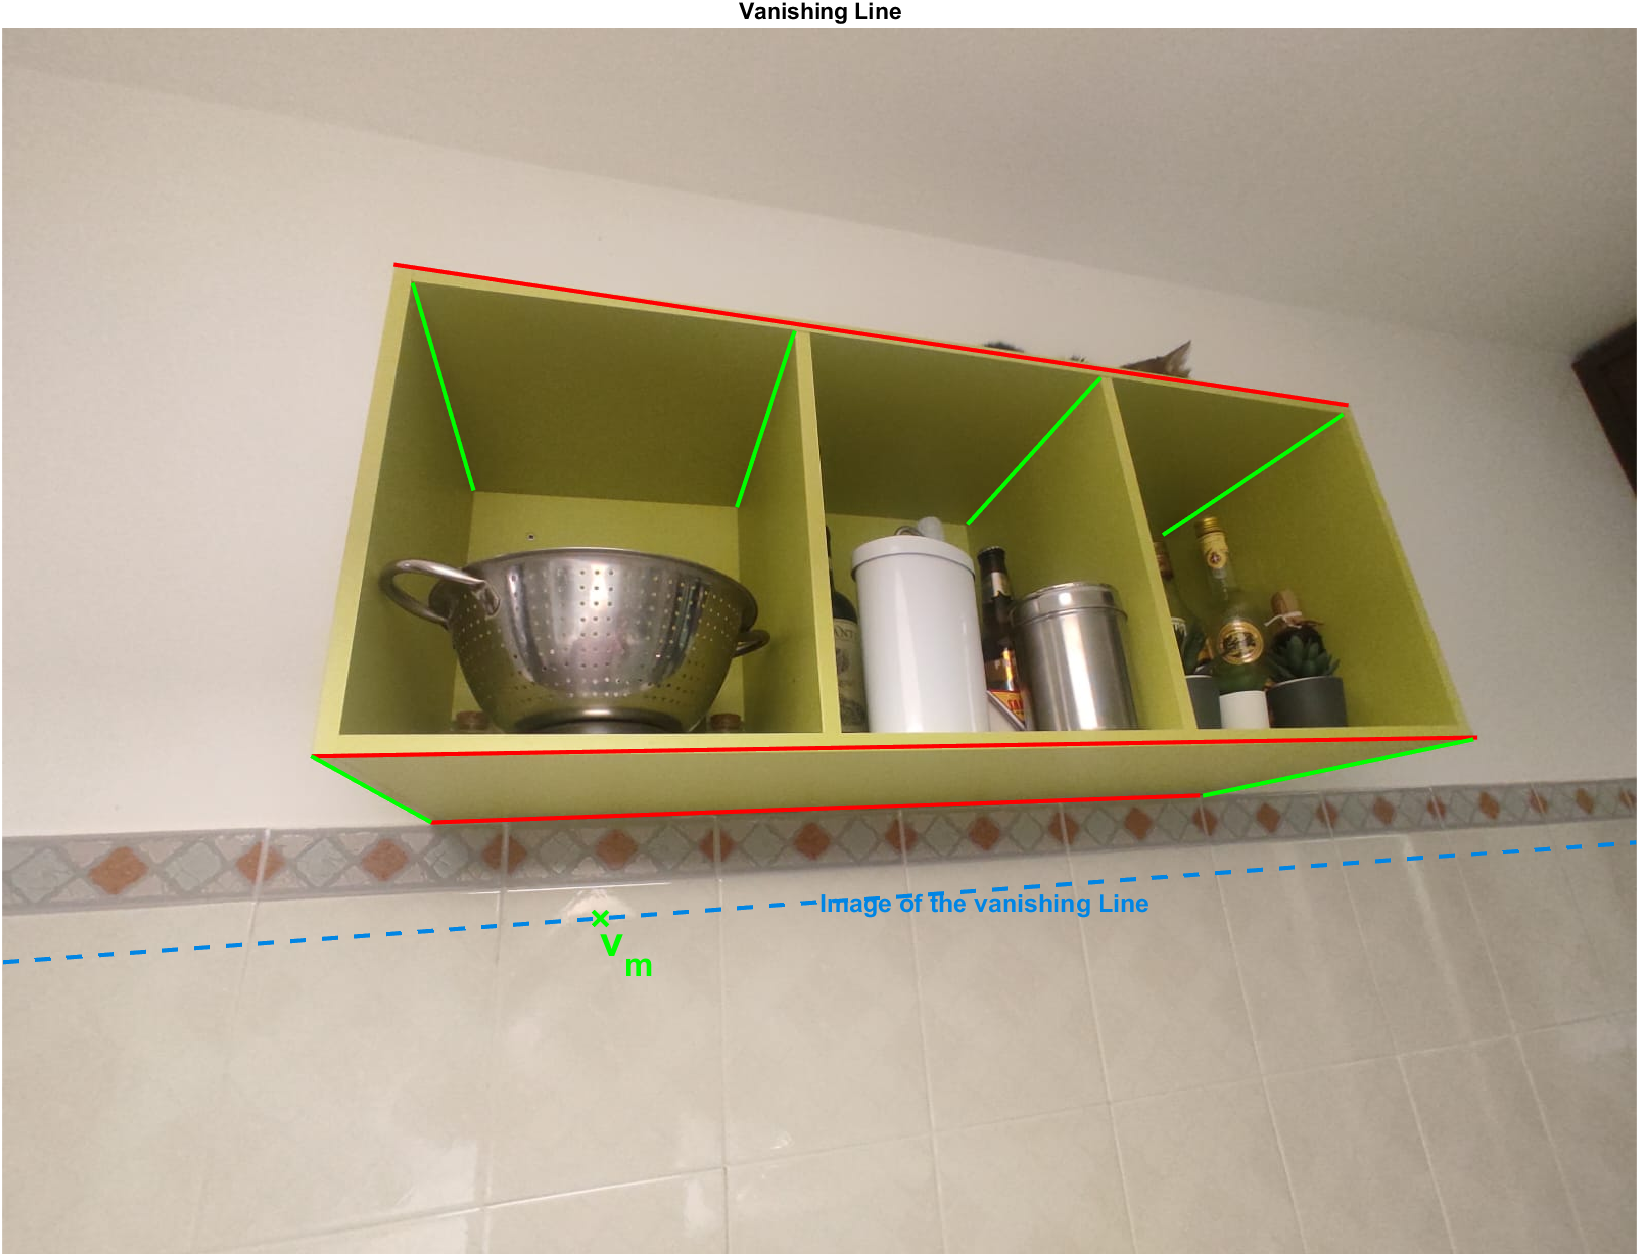
\includegraphics[height=9.5cm, width=\textwidth, keepaspectratio]{Report/Images/2.1-VanishingLine/Vanishing Line.png}
\caption{\label{fig:Vanishing Line}The Extracted image of the vanishing line}
\end{figure}


\section{Metric Rectification and depth estimation}
To rectify the upper face of the cabinet a stratified approach has been chosen. The rectification is the outcome of three steps:
\begin{enumerate}
    \item Affine Rectification
    \item Affinity to make $C$ a circle
    \item Affinity to align the axis and allign the plot (optional)
\end{enumerate}

\subsection{Affine Rectification}
The purpose of the affine rectification is to find the Homography $H_{aff}$ such that $$H_{aff}^{-T} 
 \cdot l_{\infty{}}' = l_\infty{} = \colvec{0, 0, 1}$$

 Consequently $H_{aff}$ has to be of this form:
 $$
 H_{aff} = \matrixdim{3}{3}{*, *, *, *, *, *, ,l_{\infty{}}'^T, }
 $$

 In order to make the affine reconstructed image of a more manageable size the following homography has been chosen:

  $$
 H_{aff} = \matrixdim{3}{3}{\frac{1}{10}, 0, 0, 0, \frac{1}{10}, 0,-8.0288 \cdot 10^{-05}, -0.0011, 1}
 $$

 \begin{figure}[H]
\centering
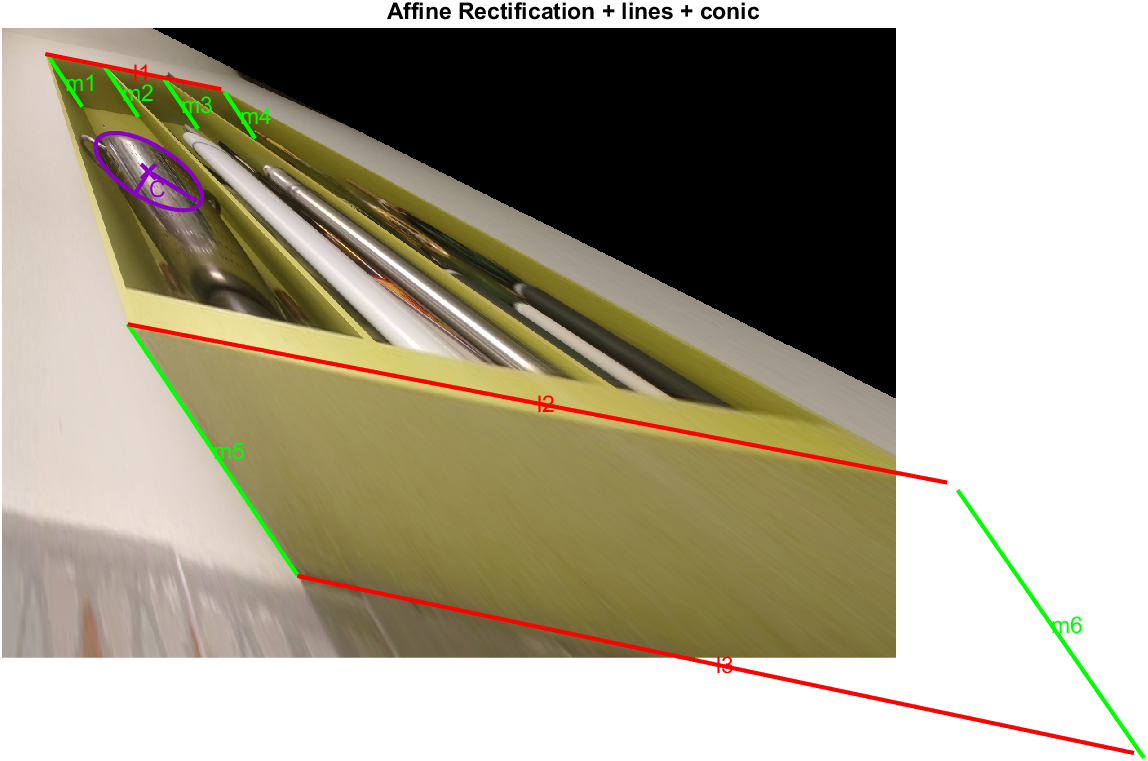
\includegraphics[height=9.5cm, width=\textwidth, keepaspectratio]{Report/Images/2.2-MetricRectification/Affine Rectification.png}
\caption{\label{fig:Affine rectification}The result of the affine rectification}
\end{figure}

\subsection{Affinity to make $C$ a circle}
Given the extracted conic $C$ in homogeneous matrix form, one can apply the affine rectification obtaining:
$$
C_{aff} = H_{aff}^{-T} \cdot C \cdot H_{aff}^{-1}
$$

From that the length ($a$ and $b$) and direction ($\theta$) of the ellipse' axis as well as the ellipse center's coordinates ($C_c$) can be extracted:

\begin{equation*}
\begin{split}
a &= 74.0106\text{ pixels}\\
b &= 31.8570\text{ pixels}\\
\theta &= 0.5529\text{ rad}\\
C_C &= \colvec{180.4210, 176.4675, 1} \text{ pixels}
\end{split}
\end{equation*}

The Homography necessary to turn $C_{aff}$ back into a circle can be factored into an isometry $U$ and a scaling $S$ as $H_{circle} = U S U^{-1}$. The two homographies can be built as follows:

\begin{equation*}
\begin{split}
U &= \matrixdim{3}{3}{\cos{\theta}, -\sin{\theta}, , \sin{\theta}, \cos{\theta}, C_c, 0, 0, }\\
S &= \matrixdim{3}{3}{1, 0, 0, 0, a/b, 0, 0, 0, 1}\\
\theta &= 0.5529\text{ rad}
\end{split}
\end{equation*}

Thus a shape reconstructing homography can be:
$$H_{metric} = H_{circle} \cdot H_{aff}$$

\subsection{Affinity to align the axis and align the plot (optional)}

To facilitate subsequent tasks another affinity is necessary to align the $l$ lines to the x-axis and to center the plot. This is encapsulated in $H_{offset}$

The final Rectifing Homography is thus:

$$H_{metric} = H_{off} \cdot H_{circle} \cdot H_{aff} = \matrixdim{3}{3}{0.1041, -0.2222, 138.2097, -0.0286, 0.1633, -14.5239, -0.0001, -0.0011, 1}$$

The result of the rectification is the following:

\begin{figure}[H]
\centering
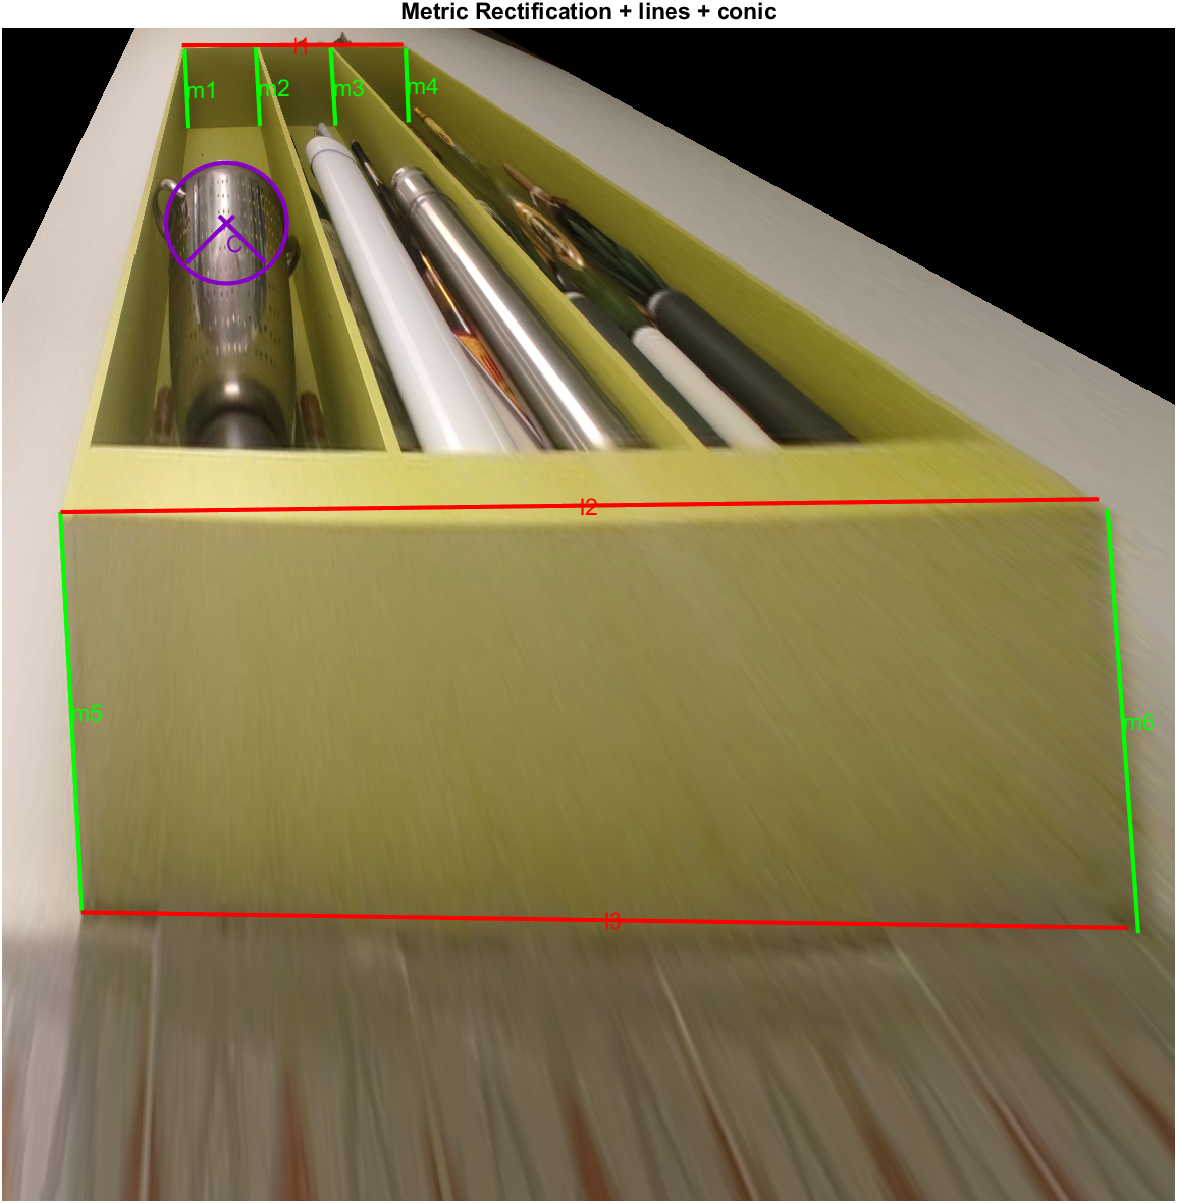
\includegraphics[height=9.5cm, width=\textwidth, keepaspectratio]{Report/Images/2.2-MetricRectification/Metric Rectification.png}
\caption{\label{fig:Metric rectification}The result of the metric rectification}
\end{figure}

\subsection{Depth estimation}
Estimating the depth $m$ is only a matter of measuring the right things. $m_5$ and $m_6$ are the only lines spanning the whole depth and they are both coplanar to $l_2$ and $l_3$ that are both 1 unit long in the scene. Since lines that share the same horizontal plane have the same scaling factor in the metric rectification, follows that by calling $m_{5_1}^m$, $m_{5_2}^m$, $m_{6_1}^m$, $m_{6_2}^m$ $l_{2_1}^m$, $l_{2_2}^m$, $l_{3_1}^m$, $l_{3_2}^m$ the homogenous coordinates of the pixel coordinated of the endpoints of the segments in the metric rectified image, the depth is:

$$
m = \frac{||m_{5_1}^m - m_{5_2}^m|| + ||m_{6_1}^m - m_{6_2}^m||}{||l_{2_1}^m - l_{2_2}^m|| + ||l_{3_1}^m - l_{3_2}^m||} = 0.39571 \text{ units} 
$$

With the exact same reasoning translated to the $m_{1:4}$ and $l_1$ lines, the internal depth of the cabinet can be computed:

$$
m_{internal} = 0.35073 \text{ units} 
$$

With this two information, the depth of the back plate of the cabinet can be estimated (This will come in handy for the 3D model reconstruction).

$$
m_{backplate} = m - m_{internal} = 0.044985 \text{ units}
$$

\section{Intrinsic Calibration}
The goal of this task is to find the calibration matrix $K$ built as follows:
$$
K = \matrixdim{3}{3}{f_x, 0, U_0, 0, f_y, V_0, 0, 0, 1}
$$

Instead of estimating $K$ directly, it is easier to find $\omega \overset{\Delta}{=} (KK^T)^{-1}$.
This matrix is built as follows:
$$
\omega = \matrixdim{3}{3}{a^2, 0, -U_0a^2, 0, 1, -V_0, -U_0a^2, -V_0, f_y^2+a^2U_0^2+V_0^2}
$$


By knowing an homography $H = [h_1, h_2, h_3]$ that goes from the coordinate on a plane $\pi$ to the image space and the vanishing point $v$ along the direction orthogonal to $\pi$, the following conditions must hold:
\begin{equation*}
\begin{split}
h_1^T\omega h_2 &= 0 \\
h_1^T\omega h_1 - h_2^T\omega h_2 &= 0\\
v^T\omega h_1 &= 0 \\
v^T\omega h_2 &= 0
\end{split}
\end{equation*}

And thus the entries of $\omega$ can be estimated as solutions of a linear system of equations.

$K$ can then be reconstructed with the Cholesky decomposition of $\omega^-1$.

In this case, the homography $H$ used is equal to $H_{metric}^{-1}$ thus setting the plane $\pi$ to be horizontal. The vanishing point $v$ can be computed with Procedure~\ref{proc:FindingIntersection} on the lines $h_{1:4}$.

The estimated calibration matrix is:
$$
K = \matrixdim{3}{3}{782.3411, 0, 800.8240, 0, 789.2100, 534.6531, 0, 0, 1}
$$

\section{Height estimation}
By multiplying $H$ with $K^{-1}$, a set of basis of $\pi$ $r1$ and $r2$ and the offset $o_\pi$ are obtained, expressed in the reference frame of the camera:
$$r_{cam} = \matrixdim{1}{3}{r_1, r_2, o_\pi} = K^{-1}H$$

These coordinates are known up to scale, which is the key for selecting planes at a given height. That's because it is known that the segments $l_{1:3}$ are 1 unit long in the scene, thus by dividing the vectors by the length of the metric rectified  $l_1^m$ ($|l_1^m|$) or $l_2^m$ ($|l_2^m|$), a set of 3D origin and coordinates of the upper and lower face of the cabinet can be found. Calling $\hat{r_3}$ a unit vector orthogonal to both $r_1$ and $r_2$, the height can be simply computed as:
$$
h = \hat{r_3}^T \cdot (\frac{o_\pi}{|l_1^m|} - \frac{o_\pi}{|l_2^m|}) = (\frac{1}{|l_1^m|} - \frac{1}{|l_2^m|}) \hat{r_3}^T \cdot o_\pi = 0.3842 \text{ units}
$$

\section{Coordinates of S}
Starting from the points of the curve in the original image expressed in homogenous coordinates in the matrix $S$. First, they need to be metric rectified obtaining $S_{metric} = H_{metric}\cdot S$. They can then be expressed in the camera 3d coordinate system as $S_{cam}' = r_{cam} \cdot S_{metric}$.

Now the appropriate scaling factor $s$ to place the points at $h/2$ needs to be found. The scaling $s$ is one such that by scaling the offset of the plane of the top face of the cabinet it moves by $h/2$ units along the $\hat{r_3}$ direction

\begin{equation*}
\begin{split}
\hat{r_3}^T \cdot(\frac{o_\pi}{|l_1^m|} - s \frac{o_\pi}{|l_1^m|}) &= h/2\\
(1 - s) &= h/2\\
s &= 1 - \frac{h\cdot |l_1^m|}{2\cdot \hat{r_3}^T \cdot o_\pi}
\end{split}
\end{equation*}

Thus $S_{cam} = s \cdot S_{cam}'$

Then the 3D coordinates of the chosen origin (the bottom left corner of the cabinet closer to the camera) must be found. Luckily, the coordinate of that point in the metric rectification is $l_{2_1}^m$, thus:

$$
O_{cam} = \frac{r_{cam} \cdot l_{2_1}^m}{|l_2^m|}
$$

The last piece is to find the $\hat{X}_{cam}$ and $\hat{Y}_{cam}$ versors in the camera space. They are aligned with $r_1$ and $r_2$.
$$
\hat{X}_{cam} = r_1 / |r1|
$$
$$
\hat{y}_{cam} = r_2 / |r2|
$$

Thus 
$$S_{XY} = \matrixdim{2}{1}{\hat{X}_{cam}^T, \hat{Y}_{cam}^T} \cdot (S_{cam} - O_{cam})$$


\begin{figure}[H]
\centering
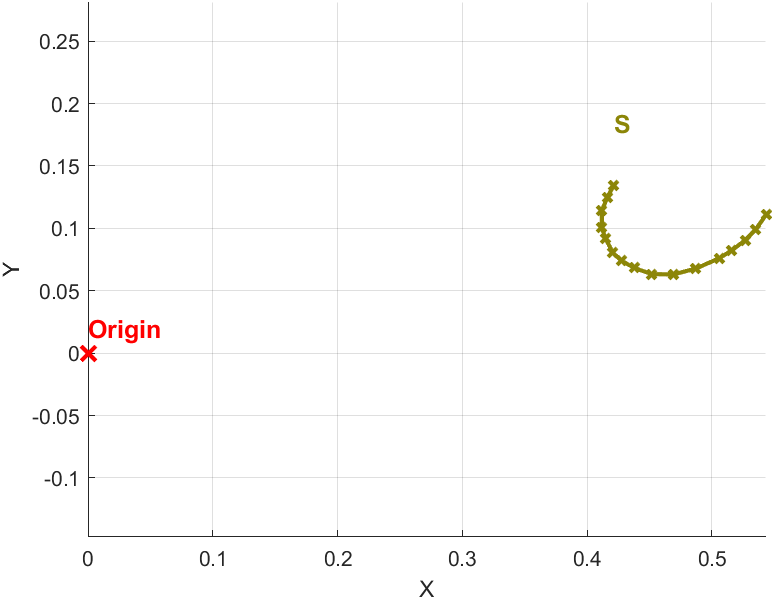
\includegraphics[height=9.5cm, width=\textwidth, keepaspectratio]{Report/Images/2.4-S_coordinated/S_coordinates.png}
\caption{\label{fig:S XY coordinate}The X Y Coordinates of S}
\end{figure}

\section{Camera Localization}
Since both the chosen origin and the chosen axis are known in the camera reference frame:

$$
R^{-1} = \matrixdim{1}{4}{\hat{X}_{cam}, \hat{Y}_{cam}, \hat{r_3}, O_{cam}}
$$

The computed $R$ matrix is:
$$
R = \matrixdim{4}{4}{0.9539, 0.0510, 0.2956, 0.1479,    -0.2924, 0.3790, 0.8780, -0.5679, -0.0673, -0.9240, 0.3765, -0.1038, 0, 0, 0, 1}
$$